\documentclass[tikz,border=10pt]{standalone}
\usepackage{pgfplots}
\pgfplotsset{compat=newest}

\colorlet{green_set}{green!70!black}
\colorlet{purple_set}{blue!80!cyan!60!red!95!black!90}
\colorlet{red_set}{red!80!black}

\begin{document}
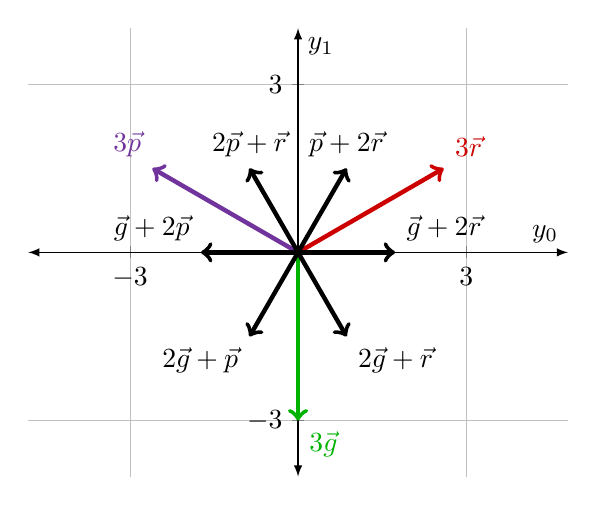
\begin{tikzpicture}
    \begin{axis}[
        axis lines=middle,
        xmin=-4, xmax=4,
        ymin=-4, ymax=4,
        xlabel={$y_0$},
        ylabel={$y_1$},
        grid=both,
        grid style={line width=.1pt, draw=gray!10},
        major grid style={line width=.2pt,draw=gray!50},
        axis line style={latex-latex},
        axis equal,
        xtick={-3, 3},
        ytick={-3, 3},
    ]

    \draw[->, ultra thick, green_set] (axis cs:0,0) -- (axis cs:0,-3) node[anchor=north west] {$3\vec{g}$};
    \draw[->, ultra thick, purple_set] (axis cs:0,0) -- (axis cs:-2.598,1.5) node[anchor=south east] {$3\vec{p}$};
    \draw[->, ultra thick, red_set] (axis cs:0,0) -- (axis cs:2.598,1.5) node[anchor=south west] {$3\vec{r}$};

    \draw[->, ultra thick, black] (axis cs:0,0) -- (axis cs:-0.866,-1.5) node[anchor=north east] {$2\vec{g}+\vec{p}$};
    \draw[->, ultra thick, black] (axis cs:0,0) -- (axis cs:0.866,-1.5) node[anchor=north west] {$2\vec{g}+\vec{r}$};

    \draw[->, ultra thick, black] (axis cs:0,0) -- (axis cs:-1.732,0) node[anchor=south east] {$\vec{g}+2\vec{p}$};
    \draw[->, ultra thick, black] (axis cs:0,0) -- (axis cs:1.732,0) node[anchor=south west] {$\vec{g}+2\vec{r}$};

    \draw[->, ultra thick, black] (axis cs:0,0) -- (axis cs:-0.866,1.5) node[anchor=south] {$2\vec{p}+\vec{r}$};
    \draw[->, ultra thick, black] (axis cs:0,0) -- (axis cs:0.866,1.5) node[anchor=south] {$\vec{p}+2\vec{r}$};

    \end{axis}
\end{tikzpicture}
\end{document}
